\documentclass[book,a4paper,12pt]{memoir}
\usepackage{listings}
\usepackage{xcolor}
\usepackage{hyperref}
\usepackage{graphicx}
\begin{document}
\definecolor{ultralightgray}{gray}{0.85}
\openany
\title{KIOS miniCPS - Matlab Manual}
\posttitle{\par\vskip1em{\normalfont\normalsize\scshape Version 0.01 \par\vfill}\end{center}}
\author{Philippos Isaia}
\date{13 December 2018}
\maketitle
\frontmatter
\tableofcontents
\chapter{Acknowledgements}
\label{cha:ack}

miniCPS was created by Daniele Antonioli as part of Security of Cyber - Physical Systems group at Singapore University of Technology and Design.
For more information visit: \\
\url{https://github.com/scy-phy} \\
\url{https://francozappa.github.io/}

\mainmatter
\chapter{Installation}
\label{cha:install}
This repository works better with Ubuntu 14.04 and VMware.  Therefore, download Ubuntu 14.04 and create a virtual machine or use native installation.  During Ubuntu installation, make sure you install OpenSSH Server.  This will be used later on in order to communicate with Mininet as well as the VM.

First of all you have to install git in order to get miniCPS repository.  To install it use the command below.

\begin{lstlisting}[backgroundcolor = \color{ultralightgray}, language = C, xleftmargin = 0.1cm, framexleftmargin = 0.3em, showstringspaces=false]
sudo apt-get install git
\end{lstlisting}

In order to clone the miniCPS git repository using the following command:
 
\begin{lstlisting}[backgroundcolor = \color{ultralightgray}, language = C, xleftmargin = 0.1cm, framexleftmargin = 0.3em, showstringspaces=false]
sudo git clone
    https://github.com/philippos-isaia/minicps.git
\end{lstlisting}

Then use the preconfigured install.sh script in order to install minicps and all its dependencies.  Use the following commands:

\begin{lstlisting}[backgroundcolor = \color{ultralightgray}, language = C, xleftmargin = 0.1cm, framexleftmargin = 0.3em, showstringspaces=false]
cd minicps
sudo sh install.sh
\end{lstlisting}

Note: The install.sh script used above has been pre-configured to update and upgrade Ubuntu as well as install dependencies such as python, mininet, xterm etc.


In order to be able to have a communication with the Virtual Machine (control/management) as well as communicate with Mininet's virtual hosts, two network interfaces will be needed.  First of all, you will have to edit the interfaces file in order to add an extra interface.  Use the command below to open the interfaces file:

\begin{lstlisting}[backgroundcolor = \color{ultralightgray}, language = C, xleftmargin = 0.1cm, framexleftmargin = 0.3em, showstringspaces=false]
sudo nano /etc/network/interfaces
\end{lstlisting}

Add the following two lines at the end of the interfaces file:

\begin{lstlisting}[backgroundcolor = \color{ultralightgray}, language = C, xleftmargin = 0.1cm, framexleftmargin = 0.3em, showstringspaces=false]
auto eth1
iface eth1 inet dhcp
\end{lstlisting}

Finally, some modification have to be performed on the VMware software.  First of all go to the appropriate VM settings, and add a Network Adapter (Figure~\ref{VMSettings}).  One of the network addapters should be ``Host-only'' wheres the other should be ``Custom''.  For the custom adapter use the appropriate NAT settings, which are defined in the next step (Figure~\ref{VMEditor}).

\begin{figure}[h!]
	\centering
	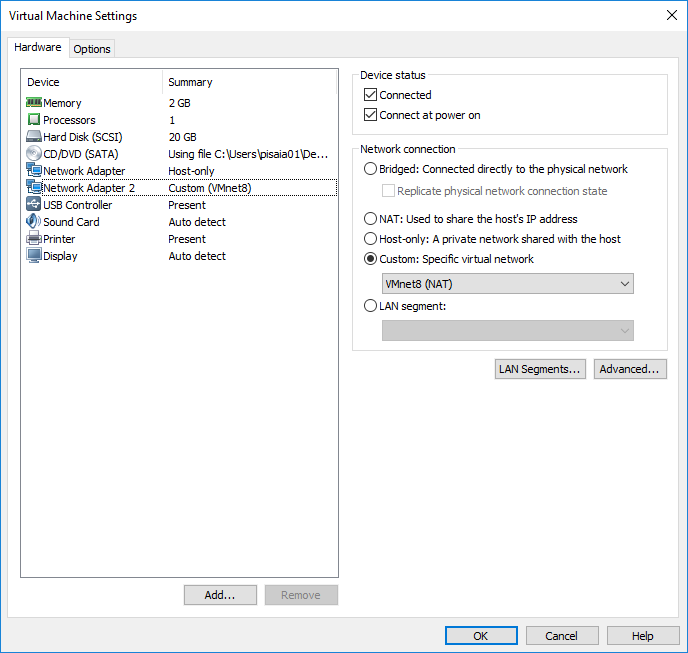
\includegraphics[scale=0.6]{VirtualMachineSettings}
	\caption{Virtual Machine Settings}
	\label{VMSettings}
\end{figure}

Lastly, go to Virtual Network Editor from within VMware nad make sure that the NAT settings are appropriate.

\begin{figure}[h!]
	\centering
	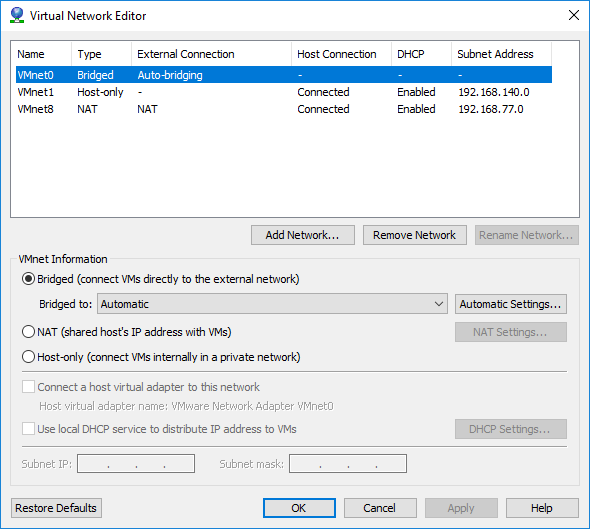
\includegraphics[scale=0.7]{VirtualNetworkEditor}
	\caption{Virtual Network Editor}
	\label{VMEditor}
\end{figure}


\chapter{Basic Use}
\label{cha:basicuse}

This version of miniCPS has some differences compared to the original one provided by Daniele Antonioli.  The main differences are around the configuration / \textbf{utils.py} file and the way miniCPS handles it as well as the way miniCPS sends and receives modbus signals.  The reason of making these changes is to allow for a faster and easier creation/deployment of topologies (plus the ability of an interactive interface in the future), as well as the ability to communicate and exchange information with Matlab modbus servers / clients.  This might need further adjustments once physical devices are added to the equation.

Please note that this version of miniCPS uses \textbf{Python 2.7}.  Depending on future projects / needs we can make it compatible with \textbf{Python 3.*}.

In the \textbf{minicps/examples} directory you can find two examples:

\begin{itemize}
  \item \textbf{basic-sc} \\ basic-sc is an empty scenario that has all the necessary files needed for you to start creating your own scenario
  \item \textbf{matlab-sc1} \\ matlab-sc1 is a scenario provided that allows the connection of minicps with matlab - simulink.  More about this scenario in Chapter~\ref{cha:matlabsc1}
\end{itemize}

In order to use miniCPS you can copy the \textbf{basic-sc1} or \textbf{matlab-sc1} scenarios and use them as a starting point or create your own scenarios from scratch .

\section{utils.py}
\label{cha:basicuse-sec:utils}
\textbf{utils.py} file acts as a configuration file.  Here all the constants are defined.  In this version of miniCPS, the topology of the network can be defined as well.

\noindent Here are examples on how to define staff in \textbf{utils.py}

\noindent Use the HOSTS variable to define all the hosts (The Coordinator, PLCs, attackers, random machines).  Do not define any switch

\begin{lstlisting}[backgroundcolor = \color{ultralightgray}, language = Python, xleftmargin = 0.1cm, framexleftmargin = 0.3em, showstringspaces=false]
HOSTS = [`coordinator', `plc1', `plc2', `attacker']
\end{lstlisting}


\noindent Use the SWITCHES variable to define the switches that are available in the emulated network

\begin{lstlisting}[backgroundcolor = \color{ultralightgray}, language = Python, xleftmargin = 0.1cm, framexleftmargin = 0.3em, showstringspaces=false]
SWITCHES = [`s1']
\end{lstlisting}

\noindent Use the NAT boolean to define if NAT will be used to assign IP addresses to all the nodes of the topology (HOSTS + SWITCHES).  If NAT is used (i.e. NAT=True), after the creation of the network, the IP addresses of all the nodes will be shown in the command line.
\begin{lstlisting}[backgroundcolor = \color{ultralightgray}, language = Python, xleftmargin = 0.1cm, framexleftmargin = 0.3em, showstringspaces=false]
NAT = True
\end{lstlisting}

\noindent Use the IP variable to define the IP addresses of all the machines (HOSTS + SWITCHES).  Note that if you are using NAT (which you should if you want seamless connectivity) then these IP addresses will not be valid and Mininet using your system's DHCP will assign new addresses to your nodes.

\begin{lstlisting}[backgroundcolor = \color{ultralightgray}, language = Python, xleftmargin = 0.1cm, framexleftmargin = 0.3em, showstringspaces=false]
IP = {
    `coordinator': `192.168.1.10'
    `plc1': `192.168.1.20',
    `plc2': `192.168.1.30',
    `attacker': `192.168.1.50',
    `s1': `172.20.81.141',
}
\end{lstlisting}


\noindent Use the NETMASKS dictionary to define the netmasks

\begin{lstlisting}[backgroundcolor = \color{ultralightgray}, language = Python, xleftmargin = 0.1cm, framexleftmargin = 0.3em, showstringspaces=false]
NETMASKS = {
    `coordinator': `/24',
    `plc1': `/24',
    `plc2': `/24',
    `attacker': `/24',
    `s1': `/24',
}
\end{lstlisting}


\noindent Use the MAC dictionary to define the MAC addresses

\begin{lstlisting}[backgroundcolor = \color{ultralightgray}, language = Python, xleftmargin = 0.1cm, framexleftmargin = 0.3em, showstringspaces=false]
MAC = {
    `coordinator': `00:1D:9C:C7:B0:30'
    `plc1': `00:1D:9C:C7:B0:70',
    `plc2': `00:1D:9C:C8:BC:46',
    `attacker': `00:1D:9C:C8:BC:48',
    `s1': `08:00:27:39:a6:83',
}
\end{lstlisting}


\noindent Use the CONNECTIONS dictionary to define the connections between HOSTS and SWITCHES.  Note that connections are bidirectional therefore define them only once.

\begin{lstlisting}[backgroundcolor = \color{ultralightgray}, language = Python, xleftmargin = 0.1cm, framexleftmargin = 0.3em, showstringspaces=false]
CONNECTIONS = {
    `coordinator': `s1',
    `plc1': `s1',
    `plc2': `s1',
    `attacker': `s1',
}
\end{lstlisting}


\noindent Define sensors and actuators as tubles

\begin{lstlisting}[backgroundcolor = \color{ultralightgray}, language = Python, xleftmargin = 0.1cm, framexleftmargin = 0.3em, showstringspaces=false]
sen_1 = (`s1', 1, `REAL')
sen_2 = (`s2', 1, `REAL')
sen_3 = (`s3', 1, `REAL')
sen_4 = (`s4', 1, `REAL')
sen_5 = (`s5', 1, `REAL')
pump_1 = (`p2', 1, `REAL')
\end{lstlisting}


\noindent Define the method used for modbus transfer plus the offset for each device (sensor / actuator) that uses modbus (both internally emulated as well as externally simulated or physically present).  Note: 
\\CO stands for 1-bit, coil, read and write
\\DI  stands for 1-bit, discrete input, read only
\\HR stands for 16-bit, holding register, read and write
\\IR stands for 16-bit, input register, read only

\begin{lstlisting}[backgroundcolor = \color{ultralightgray}, language = Python, xleftmargin = 0.1cm, framexleftmargin = 0.3em, showstringspaces=false]
SEN_1 = (`HR', 0)
SEN_2 = (`HR', 8)
SEN_3 = (`HR', 16)
SEN_4 = (`HR', 24)
SEN_5 = (`HR', 32)
\end{lstlisting}


\noindent Define PLCs details in order to initialise the server as well as assign the appropriate sensors/actuators to the appropriate PLC.  Initialising the server/client with the correct protocol allows for data exchange.  Use \textbf{enip} for EtherNet/IP and \textbf{modbus} for Modbus.  For modbus, the tags should include the amount of bits available for data transfer.

\begin{lstlisting}[backgroundcolor = \color{ultralightgray}, language = Python, xleftmargin = 0.1cm, framexleftmargin = 0.3em, showstringspaces=false]
# enip
PLC1_ADDR = IP[`plc1']
PLC1_TAGS = (sen_4, sen_5,)
PLC1_SERVER = {
    `address': PLC1_ADDR,
    `tags': PLC1_TAGS
}
PLC1_PROTOCOL = {
    `name': `enip',
    `mode': 1,
    `server': PLC1_SERVER
}

# modbus
S1_TAGS = (10, 10, 10, 100)
S1_ADDR = IP[`s1']
S1_SERVER = {
    `address': S1_ADDR,
    `tags': S1_TAGS
}
S1_PROTOCOL = {
    `name': `modbus',
    `mode': 1,
    `server': S1_SERVER
}
\end{lstlisting}


\newpage
\section{topo.py}
\label{cha:basicuse-sec:topo}
\textbf{topo.py} file is used to create the topology of the emulated ``network''.  Note that as it stands, the file uses information from the \textbf{utils.py} file in order to create the topology.  This file uses Mininet entirely, therefore it can be modified using Mininet's capabilities in order to create any topology that Mininet supports.

\noindent The default file uses the following three loops to create switches, hosts and the links between them.

\begin{lstlisting}[backgroundcolor = \color{ultralightgray}, language = Python, xleftmargin = 0.1cm, framexleftmargin = 0.3em, showstringspaces=false]
from mininet.topo import Topo
for switch in SWITCHES:
    variables[switch] = self.addSwitch(switch)

for host in HOSTS:
    variables[host] = self.addHost(host, 
            ip=IP[host]+NETMASKS[host], mac=MAC[host])

for connection in CONNECTIONS:
    self.addLink(connection, CONNECTIONS[connection])
\end{lstlisting}


\noindent The same code can be used to create custom topologies without the use of the utils.py file.

\begin{lstlisting}[backgroundcolor = \color{ultralightgray}, language = Python, xleftmargin = 0.1cm, framexleftmargin = 0.3em, showstringspaces=false]
from mininet.topo import Topo
s1=net.addSwitch(`s1')
s2=net.addSwitch(`s2')
s3=net.addSwitch(`s3')

h1 = net.addHost(`h1', ip=`10.0.0.1')
h2 = net.addHost(`h2', ip=`10.0.0.2')
h3 = net.addHost(`h3', ip=`10.0.0.3')
h4 = net.addHost(`h4', ip=`10.0.0.4')

net.addLink(s2, h1)
net.addLink(s2, h2)
net.addLink(s3, h3)
net.addLink(s3, h4)
net.addLink(s1, s2)
net.addLink(s1, s3)
\end{lstlisting}


\noindent We can even limit the CPU allocation of each node/host, or create and destroy links dynamically or at a predefined time.

\newpage
\section{run.py}
\label{cha:basicuse-sec:run}
\textbf{run.py} file essentially starts the emulation / experiment.  It starts the topology as well as the controller and the files running on each host.  These files can be Python files containing event handling / logic / etc.
We usually use the \textbf{net.pingAll()} command in order to force all the hosts/nodes that are connected to ping each other.  This allows the links to be initialised.  

\begin{lstlisting}[backgroundcolor = \color{ultralightgray}, language = Python, xleftmargin = 0.1cm, framexleftmargin = 0.3em, showstringspaces=false]
net.start()
net.pingAll()
\end{lstlisting}


\noindent In order to run code in specific hosts/nodes we can place our Python code in the proper directory (i.e. the same directory as the run.py) and run it from the code.

\begin{lstlisting}[backgroundcolor = \color{ultralightgray}, language = Python, xleftmargin = 0.1cm, framexleftmargin = 0.3em, showstringspaces=false]
plc1, plc2 = self.net.get(`plc1', `plc2')
plc1.cmd(sys.executable + `plc1.py &')
plc2.cmd(sys.executable + `plc2.py &')
\end{lstlisting}


\noindent Note that we can run any Linux command as well.  This allows us to run packet capturing softwares such as wireshark.  Note that Mininet and subsequently miniCPS run as super user.  That means each command should be modified accordingly in order to work.

\begin{lstlisting}[backgroundcolor = \color{ultralightgray}, language = Python, xleftmargin = 0.1cm, framexleftmargin = 0.3em, showstringspaces=false]
plc1 = self.net.get(`plc1')
plc1.cmd(`touch plc1-eth0.pcap')
plc1.cmd(`chmod o=rw plc1-eth0.pcap')
plc1.cmd(`tshark -ni any -w plc1-eth0.pcap &')
\end{lstlisting}


\noindent Note that depending on Linux version (this is tested on Ubuntu 14.04 LTS), there might be some problems with the Open vSwitch test controller.  In order to avoid any conflicts, we just kill the controller at the beginning of the \textbf{run.py} file.

\begin{lstlisting}[backgroundcolor = \color{ultralightgray}, language = Python, xleftmargin = 0.1cm, framexleftmargin = 0.3em, showstringspaces=false]
import os
os.system(``sudo killall ovs-testcontroller'')
\end{lstlisting}


\newpage
\section{Run the Code}
\label{cha:basicuse-sec:runthecode}
There are two ways to start an emulation / experiment.

\begin{enumerate}
\item Run the \textbf{run.py} python file as a super user.

\begin{lstlisting}[backgroundcolor = \color{ultralightgray}, language = Python, xleftmargin = 0.1cm, framexleftmargin = 0.3em, showstringspaces=false]
sudo python run.py
\end{lstlisting}


\item Edit the \textbf{Makefile} in order to add the appropriate run commands and then use make in the miniCPS directory to run it (i.e. \textbf{``make PROJECT\_NAME''})

\begin{lstlisting}[backgroundcolor = \color{ultralightgray}, language = Python, xleftmargin = 0.1cm, framexleftmargin = 0.3em, showstringspaces=false]
Makefile
matlab-sc1:
cd examples/matlab-sc1; $(PYTHON) 
        $(PYTHON_OPTS) run.py; cd ../..
\end{lstlisting}
\end{enumerate}

\chapter{Matlab Scenario 1}
\label{cha:matlabsc1}

This is an example scenario that shows how the connection between miniCPS and Matlab/Simulink is achieved.  There are some steps that need to be followed in order for this experiment to work.

\section{Preparation}
\label{cha:basicuse-sec:prepare}

If you are running miniCPS in a virtualized environment (i.e. VMware Workstation, Oracle VM VirtualBox) then in the network settings, the network adapters should be \textbf{Enabled} and configured accordingly.  Depending on the software/method used you will have to fix this accordingly.   

You should have Matlab and Simulink installed.  Download the \textbf{matlab-sc1-model} folder from github and load it into Matlab.  Open the model file in Simulink.  In the simulink window, press on the \textbf{Simulation} tab and choose \textbf{Pacing Options}.  \textbf{Enable} pacing in order to slow down the simulation.  This allows the simulation to run with near real-time behaviour.

Start the virtual machine that hosts miniCPS and run the scenario.  To run it, under the \textbf{minicps} directory run the command
\begin{lstlisting}[backgroundcolor = \color{ultralightgray}, language = Python, xleftmargin = 0.1cm, framexleftmargin = 0.3em, showstringspaces=false]
make matlab-sc1
\end{lstlisting}

\section{Description}
\label{cha:basicuse-sec:description}

\begin{figure}[h!]
	\centering
	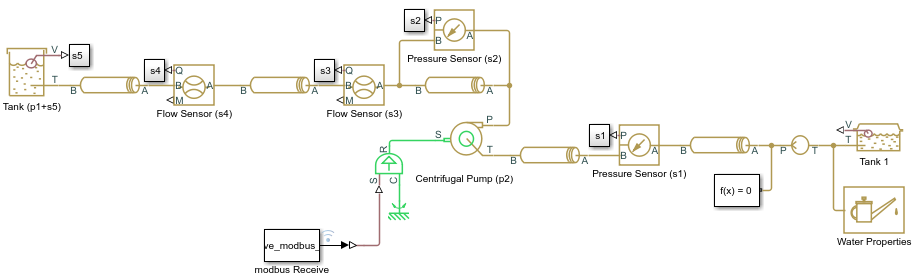
\includegraphics[scale=0.8, angle=90]{SimulinkScenario}
	\caption{Simulink Scenario Model}
\end{figure}


%\chapter{Extended Use}
%\label{cha:extendeduse}

\chapter{Docker}
\label{cha:docker}
To be created after version 0.01 is evaluated and finalised

\begin{lstlisting}[backgroundcolor = \color{ultralightgray}, language = Python, xleftmargin = 0.1cm, framexleftmargin = 0.3em, showstringspaces=false]

\end{lstlisting}

\backmatter

\end{document}